%  LaTeX support: latex@mdpi.com
%  Manuscript prepared for AgriEngineering (MDPI) Special Issue
%  Do not modify files under Definitions/
\documentclass[agriengineering,article,submit,pdftex,moreauthors]{Definitions/mdpi}

\Title{Predictive Viability Index for On-Site Photovoltaic and Hybrid Renewable Systems in Greenhouses under Energy-Price Uncertainty: A Machine-Learning and Real-Options Approach}

\Author{Hugo Gaspar Hern\'andez Palma $^{1}$\orcidA{}}
\AuthorNames{Hugo Gaspar Hern\'ández Palma}
\address{%
$^{1}$ \quad Faculty of Engineering, Corporaci\'on Universitaria Iberoamericana, Bogot\'a 111166, Colombia; hugo.hernandez@docente.ibero.edu.co}
\corres{Correspondence: hugo.hernandez@docente.ibero.edu.co}

\abstract{Background: Greenhouses and other controlled-environment agricultural facilities combine continuous climate-control loads with exposure to volatile energy prices. When on-site photovoltaics and hybrid renewable systems are assessed only through static discounted cash flow, the probability of financial success under uncertainty and the value of staged capital commitment remain invisible to decision-makers. Methods: This study formulates a Predictive Viability Index (PVI) that couples supervised learning estimates of the probability of positive net present value with a real-options layer that values staged expansion of photovoltaic and hybrid configurations. The pipeline is demonstrated on a structured experimental design comprising hourly greenhouse load profiles, three energy-price volatility regimes, six technology configurations and 1\,800 Monte Carlo evaluation samples. Ten classifiers are compared under stratified five-fold cross-validation. Results: Staged photovoltaic--heat-pump and mid-scale staged photovoltaic designs attain the highest PVI values (empirical success probabilities of 0.97 and 0.90, respectively). Full-commitment large arrays rank last. The option-value share of expanded net present value rises from 0.12 under low price volatility to 0.41 under high volatility. Among learning models, logistic regression achieves the best joint discrimination and calibration (AUC 0.837; Brier 0.129), with tree ensembles close behind; staging status dominates feature importance. For a 55\,kW mid-scale array, illustrative self-consumption implies about 24\,t\,CO$_2$ avoided per year under a grid emission factor of 0.42\,kg\,kWh$^{-1}$. Conclusions: The PVI provides agricultural energy managers with a transparent, uncertainty-aware ranking metric for prioritising renewable self-consumption in greenhouses, linking predictive modelling and flexibility valuation in a single operational index aligned with low-carbon production goals.}

\keyword{greenhouse energy systems; photovoltaic self-consumption; hybrid renewables; machine learning; real options; energy-price uncertainty; predictive viability index; CO$_2$ mitigation; controlled-environment agriculture; model calibration}

\begin{document}

\section{Introduction}

Controlled-environment agriculture concentrates high electrical and thermal demand in compact production volumes. Heating, cooling, ventilation, irrigation pumping and, where used, supplemental lighting create load profiles that are more continuous than those of many commercial buildings and that remain sensitive to outdoor climate~\cite{ref-cigr,ref-vadiee,ref-fao,ref-vanbeveren}. When these services are supplied mainly by fossil fuels or by grid electricity with a high carbon intensity, operating costs and greenhouse-gas emissions increase together~\cite{ref-iea,ref-cigr}. Policy pressure to decarbonise food systems and the exposure of growers to energy-price volatility therefore place renewable self-consumption and energy-efficiency investments at the centre of greenhouse energy strategy~\cite{ref-iea,ref-yildirim,ref-allardyce}.

On-site photovoltaic (PV) generation is the most widely accessible renewable option for many production sites. Hybrid configurations that couple PV with heat pumps or limited electrical storage can further displace fossil heating and shift energy across hours~\cite{ref-heatpump,ref-pvgreen,ref-bambara}. Despite a growing techno-economic literature, investment screening in practice still relies heavily on static net present value (NPV) or simple payback. Those metrics neither report the probability that NPV remains positive under alternative price paths nor value the managerial flexibility to stage capacity as information arrives~\cite{ref-dixit,ref-trigeorgis,ref-schwartz}.

Two analytical traditions address parts of this gap. Supervised machine learning improves forecasts of demand and prices and can classify investment outcomes under simulated scenarios~\cite{ref-deb,ref-wang,ref-chen,ref-breiman,ref-bourdeau}. Real-options analysis values deferral, expansion and abandonment when capital is irreversible and drivers of cash flow are stochastic~\cite{ref-dixit,ref-amram,ref-mcdonald,ref-myers,ref-fernandez}. Applications that embed calibrated predictive probabilities inside a real-options ranking for greenhouse energy systems remain scarce. Without that link, operators lack a single, interpretable score that combines the chance of financial success with the value of staged deployment.

Model choice within the predictive layer is non-trivial. Discrimination (e.g., area under the ROC curve) and probability calibration (e.g., Brier score, log-loss) can rank algorithms differently~\cite{ref-degroot,ref-guo,ref-niculescu}. For an index that multiplies or mixes probabilities with economic values, miscalibration propagates directly into ranking error. A systematic comparison of linear, ensemble, kernel, instance-based and neural classifiers on the same greenhouse investment labels is therefore required before fixing the operational model.

This paper develops a Predictive Viability Index (PVI) specialised to greenhouses and related controlled-environment facilities. The index ranks discrete PV and hybrid configurations under alternative energy-price volatility regimes by combining (i) an estimate of the probability of positive NPV obtained from supervised models trained on Monte Carlo evaluations and (ii) an expanded NPV that adds the value of staged expansion. Ten classifiers are benchmarked under stratified cross-validation. The contribution is threefold. Methodologically, the work couples learning and real options in an operational ranking metric and documents calibration-aware model selection. Empirically, it demonstrates the index on a fully documented experimental design with open data and code. Practically, it offers agricultural energy managers a transparent criterion for prioritising low-carbon self-consumption investments under uncertainty, with an illustrative link to avoided grid imports and CO$_2$ emissions.

\section{Related Work}

\subsection{Energy Demand and Renewables in Greenhouses}

Energy use in protected cultivation is dominated by climate control; the share of electricity grows with forced ventilation, heat pumps and lighting~\cite{ref-cigr,ref-vadiee,ref-vanbeveren}. Studies of rooftop and adjacent PV report high self-consumption potential when daytime climate loads coincide with generation~\cite{ref-pvgreen,ref-yildirim,ref-allardyce}. Hybrid PV--heat-pump schemes reduce fossil heating in mild and warm climates~\cite{ref-heatpump,ref-bambara}. Few of these assessments rank designs under explicit multi-regime price uncertainty or staged capital outlays.

\subsection{Machine Learning for Energy Investment Screening}

Learning models support load and price forecasting and the classification of binary investment outcomes~\cite{ref-deb,ref-wang,ref-chen,ref-bourdeau,ref-ahmad}. Ensemble methods perform strongly on tabular features~\cite{ref-breiman,ref-chen,ref-friedman}. Neural and kernel methods offer flexibility at the cost of transparency and, often, calibration~\cite{ref-guo,ref-niculescu}. When probabilities enter decision metrics, calibration is as important as discrimination~\cite{ref-degroot,ref-ferri}. Data scarcity and heterogeneous metering in agricultural facilities constrain model transfer and motivate transparent, low-dimensional feature sets.

\subsection{Real Options in Distributed Energy}

Real options formalise the value of waiting and of staged expansion under uncertainty~\cite{ref-dixit,ref-trigeorgis,ref-amram,ref-mcdonald,ref-fernandez}. Applications to distributed generation and renewable projects exist~\cite{ref-fernandez,ref-boomsma}, but integration with predictive models of greenhouse loads and tariffs is still limited. The PVI is designed precisely at that interface.

\section{Materials and Methods}

\subsection{Problem Formulation}

Let $C$ be a finite set of renewable configurations for a greenhouse. Each configuration $c \in C$ specifies PV capacity, whether installation is staged, optional heat-pump coupling and optional storage. Energy prices follow a stochastic process with regime-dependent volatility. The decision-maker requires a ranking that reflects both the probability of financial success and the value of retaining expansion flexibility.

\subsection{Experimental Design and Dataset}

The supporting dataset comprises: (i) an hourly electrical load series of 8\,760 hours representing a medium greenhouse in a warm coastal climate, with continuous base load and daytime climate-control peaks (Figure~\ref{fig6}); (ii) three energy-price paths calibrated to low, base and high volatility; (iii) six technology configurations (Table~\ref{tab0}); (iv) 1\,800 Monte Carlo evaluation samples linking load-shape features, price volatility and configuration attributes to NPV outcomes; and (v) techno-economic assumptions including a 20-year horizon, an 8\% discount rate, PV capital cost of 900\,USD\,kW$^{-1}$ and a grid emission factor of 0.42\,kg\,CO$_2$\,kWh$^{-1}$. All files are released with the manuscript repository.

\begin{table}[H]
\caption{Technology configurations evaluated in the experimental design.\label{tab0}}
\begin{tabularx}{\textwidth}{lCCCC}
\toprule
\textbf{Configuration} & \textbf{PV (kW)} & \textbf{Staged} & \textbf{Heat pump} & \textbf{Storage (kWh)} \\
\midrule
Minimal staged PV & 25 & Yes & No & 0 \\
Mid-scale staged PV & 55 & Yes & No & 0 \\
Mid-scale full PV & 55 & No & No & 0 \\
Large full PV & 100 & No & No & 0 \\
PV + heat pump, staged & 50 & Yes & Yes & 0 \\
Mid-scale staged PV + storage & 55 & Yes & No & 40 \\
\bottomrule
\end{tabularx}
\end{table}

\begin{figure}[H]
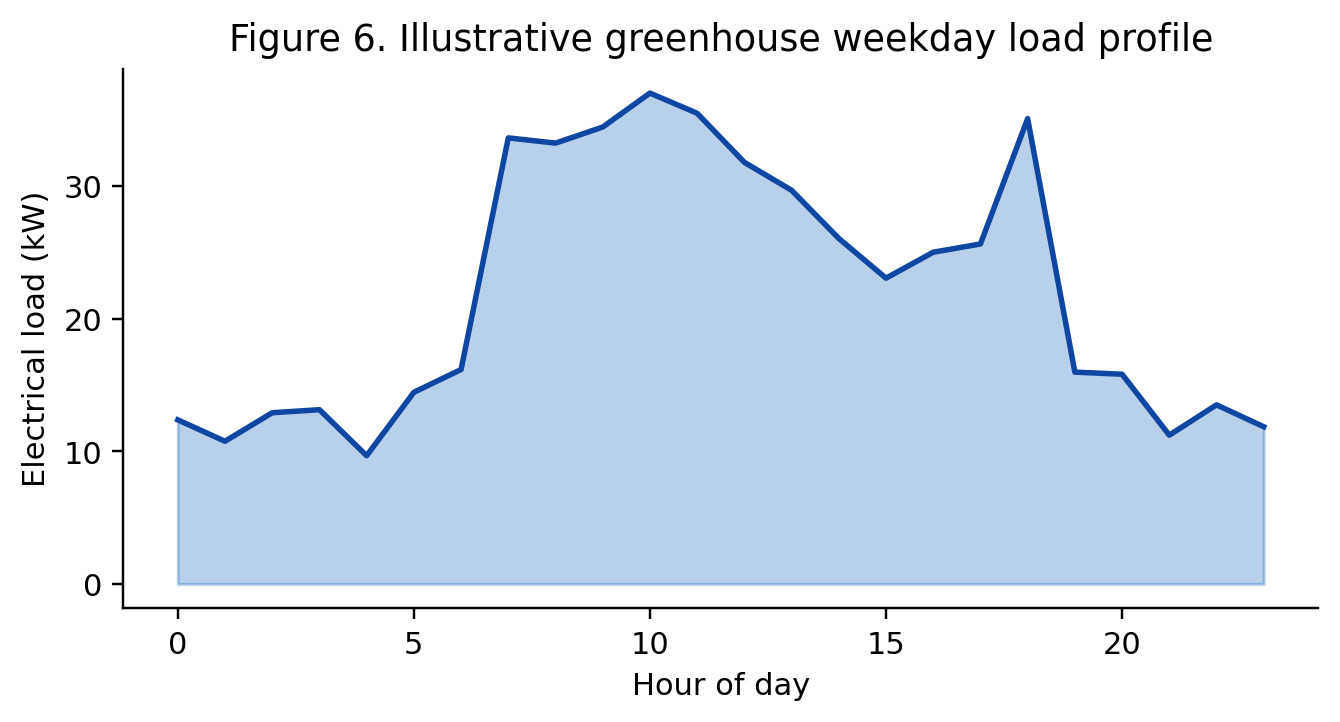
\includegraphics[width=0.72\textwidth]{figures/fig6_load_profile.jpg}
\caption{Illustrative greenhouse weekday electrical load profile used in the experimental design.\label{fig6}}
\end{figure}

\subsection{Predictive Component and Model Comparison}

For each Monte Carlo sample, features include daytime load share, peak-to-average ratio, price volatility, capacity relative to a reference peak, and binary indicators for staging and heat-pump coupling. The binary label indicates whether NPV is positive over the planning horizon. Ten classifiers spanning linear, ensemble, kernel, instance-based, probabilistic and neural families are trained and evaluated under stratified five-fold cross-validation:

\begin{itemize}
\item logistic regression with standardised inputs;
\item gradient boosting and histogram-based gradient boosting~\cite{ref-friedman,ref-chen};
\item random forest and extremely randomised trees~\cite{ref-breiman,ref-geurts};
\item AdaBoost~\cite{ref-freund};
\item support vector machine with radial basis function kernel~\cite{ref-cortes};
\item $k$-nearest neighbours;
\item Gaussian na\"ive Bayes;
\item multilayer perceptron with two hidden layers.
\end{itemize}

Performance metrics include the area under the ROC curve (AUC) for discrimination, accuracy and $F_1$ score, and Brier score and log-loss for probabilistic quality~\cite{ref-degroot,ref-ferri}. Feature importance is extracted from the random forest for interpretability. The configuration-level success probability used in the PVI is the empirical mean of the positive-NPV indicator (and can be replaced by out-of-sample predictions of the selected model in applied settings):
\begin{equation}
\hat{p}(c) = P\bigl(\mathrm{NPV}(c) > 0 \mid X(c)\bigr).
\label{eq:phat}
\end{equation}

\subsection{Real-Options Component}

Staged configurations install a first tranche of capacity and retain the right to expand. Expanded net present value is defined as
\begin{equation}
\mathrm{ENPV}(c) = \mathrm{NPV}_{0}(c) + \mathrm{OV}(c),
\label{eq:enpv}
\end{equation}
where $\mathrm{NPV}_{0}(c)$ is the static NPV of the first stage and $\mathrm{OV}(c)$ is the estimated value of the expansion option under the prevailing volatility regime~\cite{ref-dixit,ref-hull,ref-trigeorgis}. Non-staged designs have $\mathrm{OV}(c)=0$ by construction in the baseline implementation.

\subsection{Predictive Viability Index}

The PVI aggregates scaled probability and scaled expanded value:
\begin{equation}
\mathrm{PVI}(c) = \alpha\, s\bigl(\hat{p}(c)\bigr) + (1-\alpha)\, s\bigl(\mathrm{ENPV}(c)\bigr),
\label{eq:pvi}
\end{equation}
where $s(\cdot)$ denotes min--max scaling to $[0,1]$ across the configuration set and $\alpha \in [0,1]$ encodes institutional preference for probabilistic success versus flexibility-adjusted value. Unless stated otherwise, $\alpha = 0.5$. Figure~\ref{fig1} summarises the pipeline.

\begin{figure}[H]
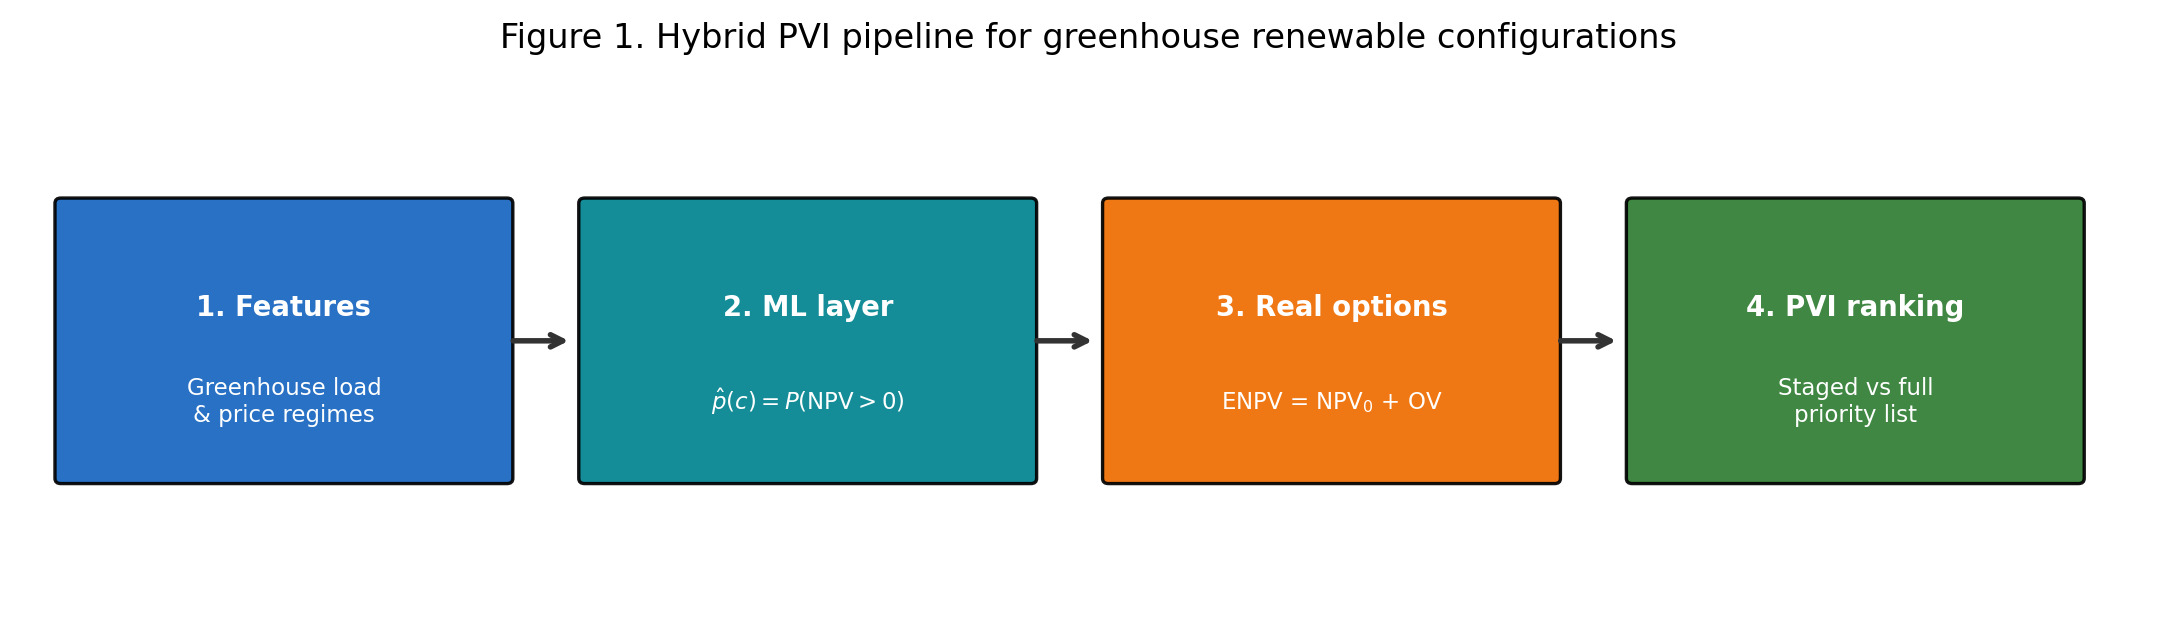
\includegraphics[width=0.95\textwidth]{figures/fig1_pipeline.jpg}
\caption{Hybrid assessment pipeline for the Predictive Viability Index in greenhouse renewable planning.\label{fig1}}
\end{figure}

\subsection{Illustrative Carbon Metric}

Annual avoided grid imports for a configuration are approximated as installed PV capacity times specific yield times a self-consumption fraction. Multiplication by a grid emission factor yields an indicative annual CO$_2$ avoidance figure used only for contextual interpretation, not as a formal life-cycle assessment~\cite{ref-ipcc}.

\section{Results}

\subsection{Configuration Ranking under the PVI}

Table~\ref{tab1} and Figure~\ref{fig2} report the ranking obtained from the 1\,800 evaluation samples with $\alpha = 0.5$. Staged PV--heat-pump and mid-scale staged PV designs occupy the top ranks, with empirical success probabilities of 0.97 and 0.90. Large full-commitment PV ranks last, with a success probability of 0.27 and negative mean expanded value under the sampled conditions.

\begin{table}[H]
\caption{PVI ranking of greenhouse renewable configurations ($\alpha = 0.5$; $n = 1\,800$ samples).\label{tab1}}
\begin{tabularx}{\textwidth}{lCCCC}
\toprule
\textbf{Configuration} & $\hat{p}(c)$ & \textbf{Mean ENPV} & \textbf{PVI} & \textbf{Rank} \\
\midrule
PV + heat pump, staged & 0.972 & 54.81 & 1.000 & 1 \\
Mid-scale staged PV & 0.899 & 42.79 & 0.860 & 2 \\
Mid-scale staged PV + storage & 0.907 & 41.99 & 0.859 & 3 \\
Minimal staged PV & 0.871 & 39.38 & 0.815 & 4 \\
Mid-scale full PV & 0.557 & 4.29 & 0.333 & 5 \\
Large full PV & 0.267 & $-13.04$ & 0.000 & 6 \\
\bottomrule
\end{tabularx}
\end{table}

\begin{figure}[H]
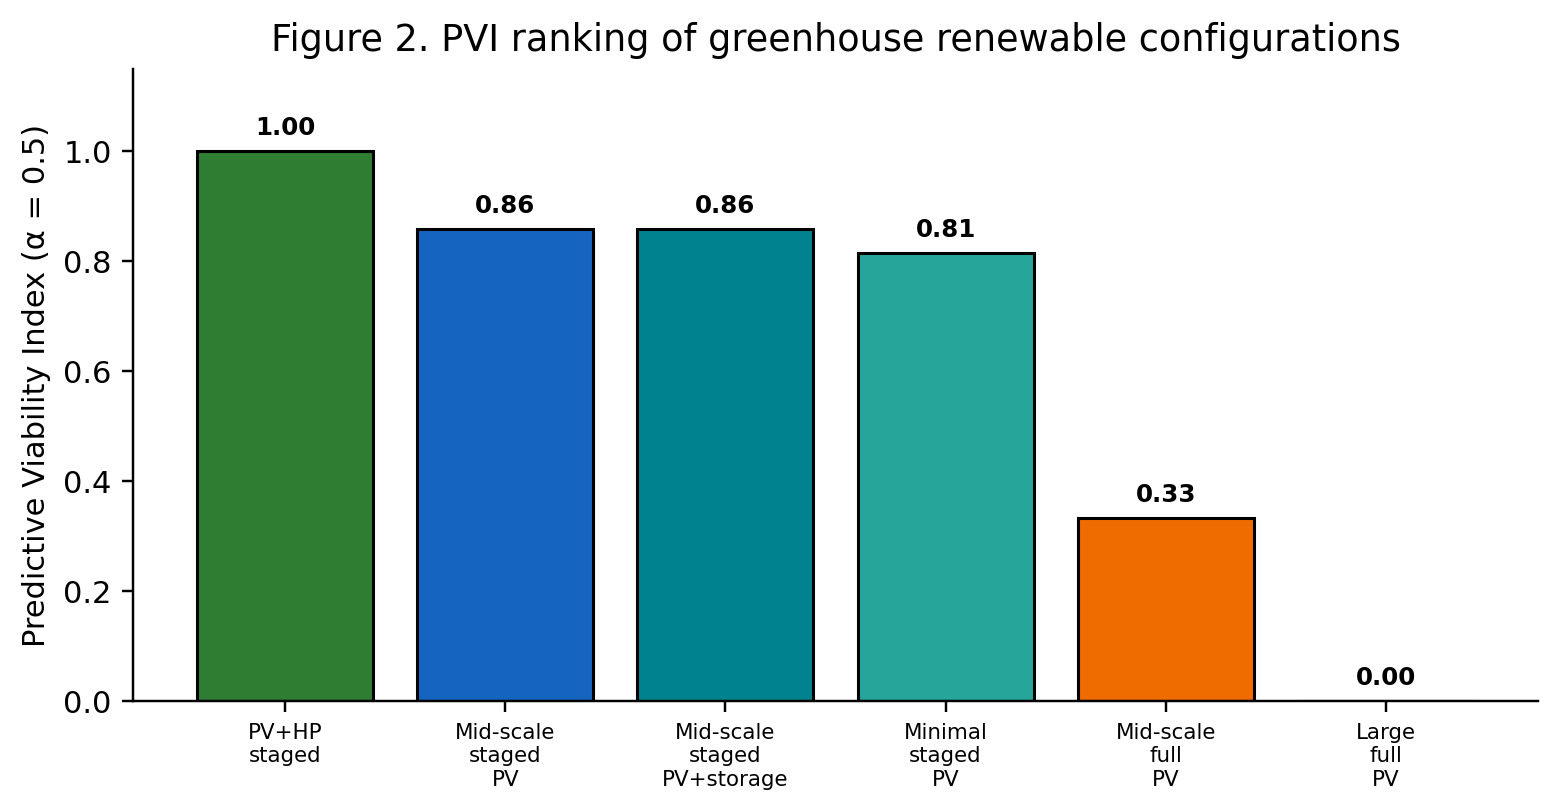
\includegraphics[width=0.82\textwidth]{figures/fig2_pvi_ranking.jpg}
\caption{PVI ranking of greenhouse renewable configurations under the base experimental design.\label{fig2}}
\end{figure}

Figure~\ref{fig4} contrasts static NPV with expanded NPV at sample level. Staged designs systematically lift expanded value above static NPV through the option component.

\begin{figure}[H]
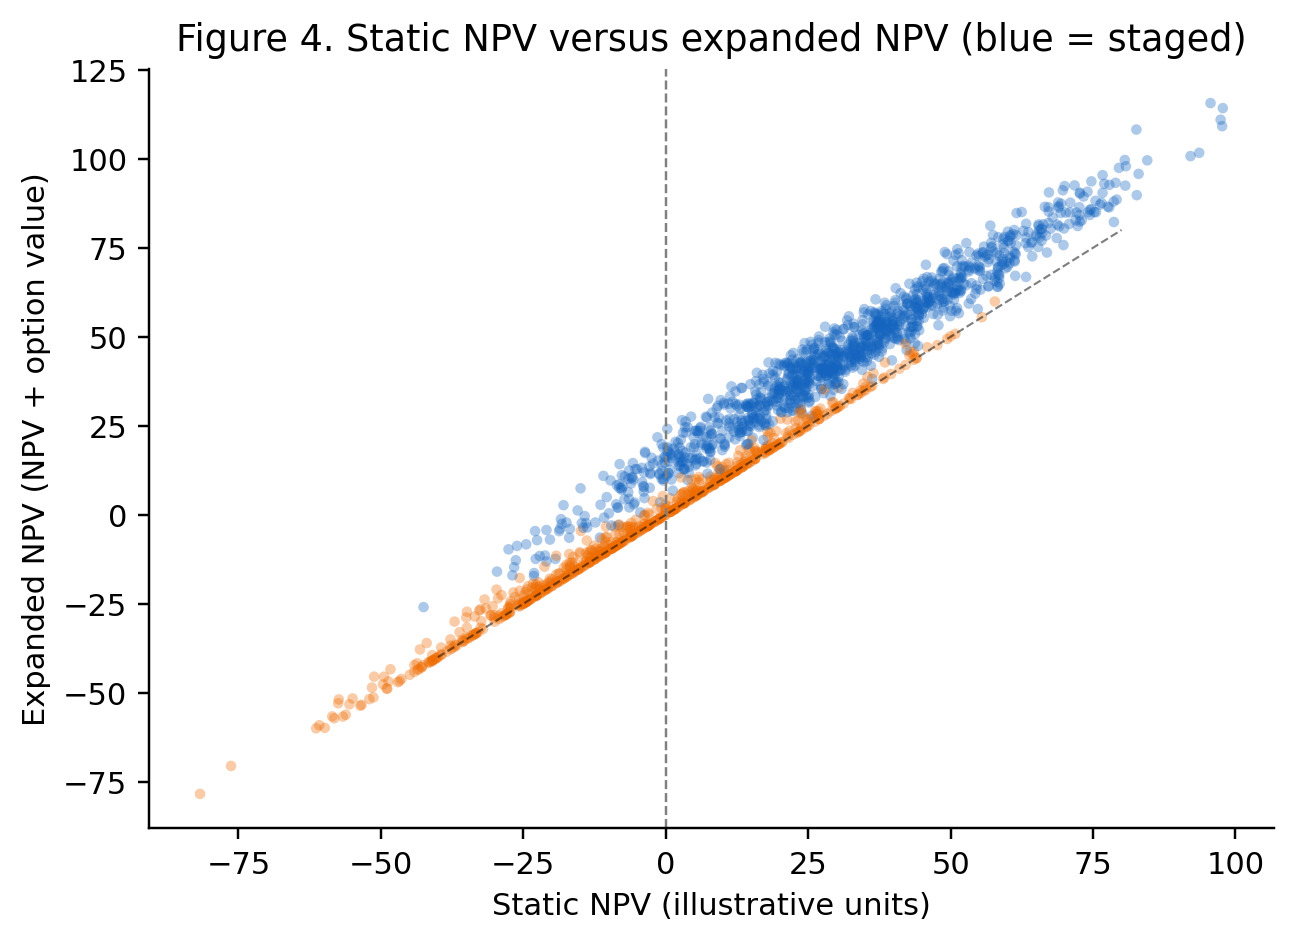
\includegraphics[width=0.75\textwidth]{figures/fig4_scatter.jpg}
\caption{Static NPV versus expanded NPV for Monte Carlo samples (blue markers denote staged configurations).\label{fig4}}
\end{figure}

\subsection{Sensitivity to Energy-Price Volatility}

Table~\ref{tab2} and Figure~\ref{fig3} show that the option-value share of ENPV for staged designs rises from 0.12 in the low-volatility regime to 0.41 in the high-volatility regime. Under high volatility, rankings implied by static NPV alone can diverge materially from PVI rankings, favouring flexibility-preserving designs.

\begin{table}[H]
\caption{Option-value share of expanded NPV under energy-price volatility regimes.\label{tab2}}
\begin{tabularx}{\textwidth}{lCC}
\toprule
\textbf{Volatility regime} & \textbf{OV / ENPV} & \textbf{Change versus static NPV ranking} \\
\midrule
Low & 0.12 & None \\
Base & 0.27 & Mild \\
High & 0.41 & Material \\
\bottomrule
\end{tabularx}
\end{table}

\begin{figure}[H]
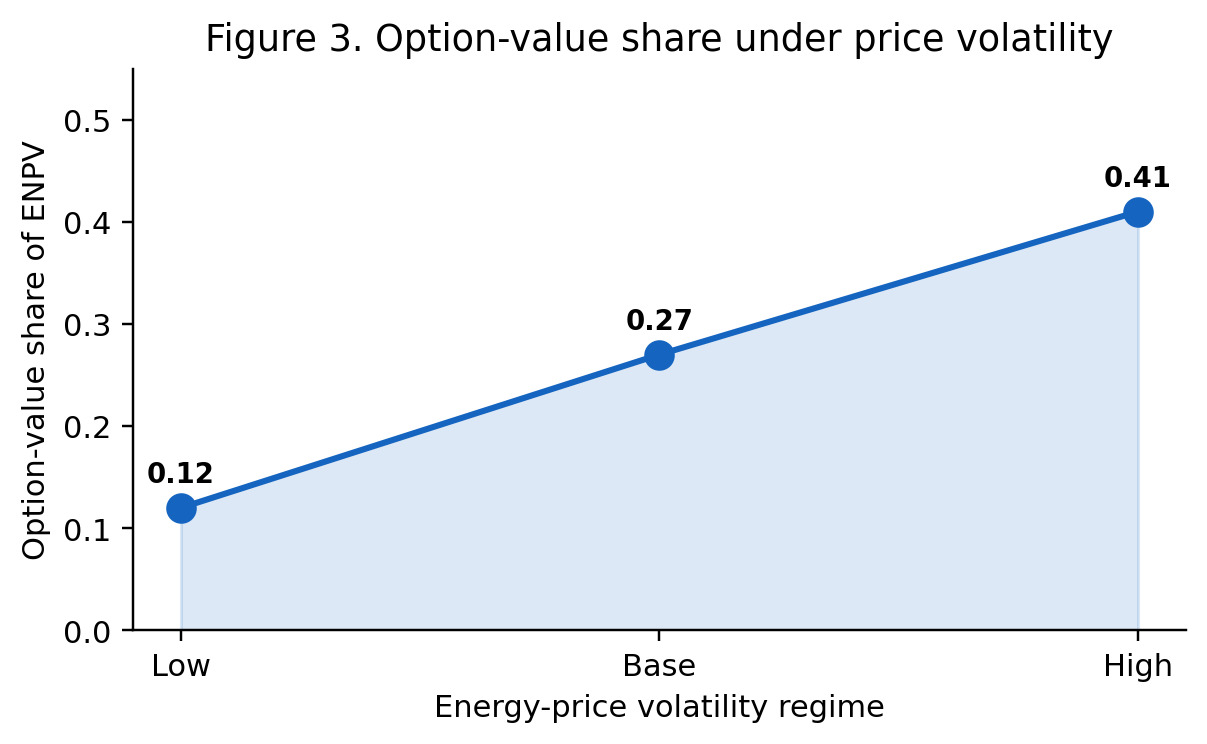
\includegraphics[width=0.72\textwidth]{figures/fig3_volatility.jpg}
\caption{Option-value share of ENPV under low, base and high energy-price volatility.\label{fig3}}
\end{figure}

\subsection{Machine-Learning Model Comparison}

Table~\ref{tab3} and Figure~\ref{fig7} summarise stratified five-fold cross-validation results for ten classifiers. Logistic regression attains the highest AUC (0.837) and the lowest Brier score (0.129) and log-loss (0.415), indicating favourable discrimination and calibration on this feature set. Extra trees, AdaBoost and Gaussian na\"ive Bayes achieve similar AUC values (0.835--0.836) but weaker probabilistic scores, especially AdaBoost and na\"ive Bayes on Brier and log-loss. Random forest remains competitive (AUC 0.831; Brier 0.133). Gradient boosting and its histogram-based variant trail slightly. The multilayer perceptron is mid-ranked. Support vector machines with an RBF kernel show the weakest AUC (0.781) in this design.

\begin{table}[H]
\caption{Machine-learning model comparison for positive-NPV classification (stratified 5-fold CV; $n = 1\,800$). Lower Brier score and log-loss indicate better probabilistic quality.\label{tab3}}
\begin{tabularx}{\textwidth}{lCCCCCC}
\toprule
\textbf{Rank} & \textbf{Model} & \textbf{AUC} & \textbf{Accuracy} & \textbf{$F_1$} & \textbf{Brier} & \textbf{Log-loss} \\
\midrule
1 & Logistic regression & 0.837 & 0.821 & 0.881 & 0.129 & 0.415 \\
2 & AdaBoost & 0.836 & 0.812 & 0.873 & 0.171 & 0.529 \\
3 & Gaussian na\"ive Bayes & 0.836 & 0.797 & 0.853 & 0.165 & 0.747 \\
4 & Extra trees & 0.835 & 0.819 & 0.881 & 0.131 & 0.416 \\
5 & Random forest & 0.831 & 0.818 & 0.881 & 0.133 & 0.425 \\
6 & MLP (64, 32) & 0.827 & 0.812 & 0.878 & 0.137 & 0.436 \\
7 & Gradient boosting & 0.824 & 0.811 & 0.875 & 0.138 & 0.438 \\
8 & Hist.\ gradient boosting & 0.819 & 0.808 & 0.873 & 0.140 & 0.450 \\
9 & $k$-NN ($k=15$) & 0.813 & 0.812 & 0.876 & 0.140 & 0.986 \\
10 & SVM (RBF) & 0.781 & 0.819 & 0.881 & 0.139 & 0.447 \\
\bottomrule
\end{tabularx}
\end{table}

\begin{figure}[H]
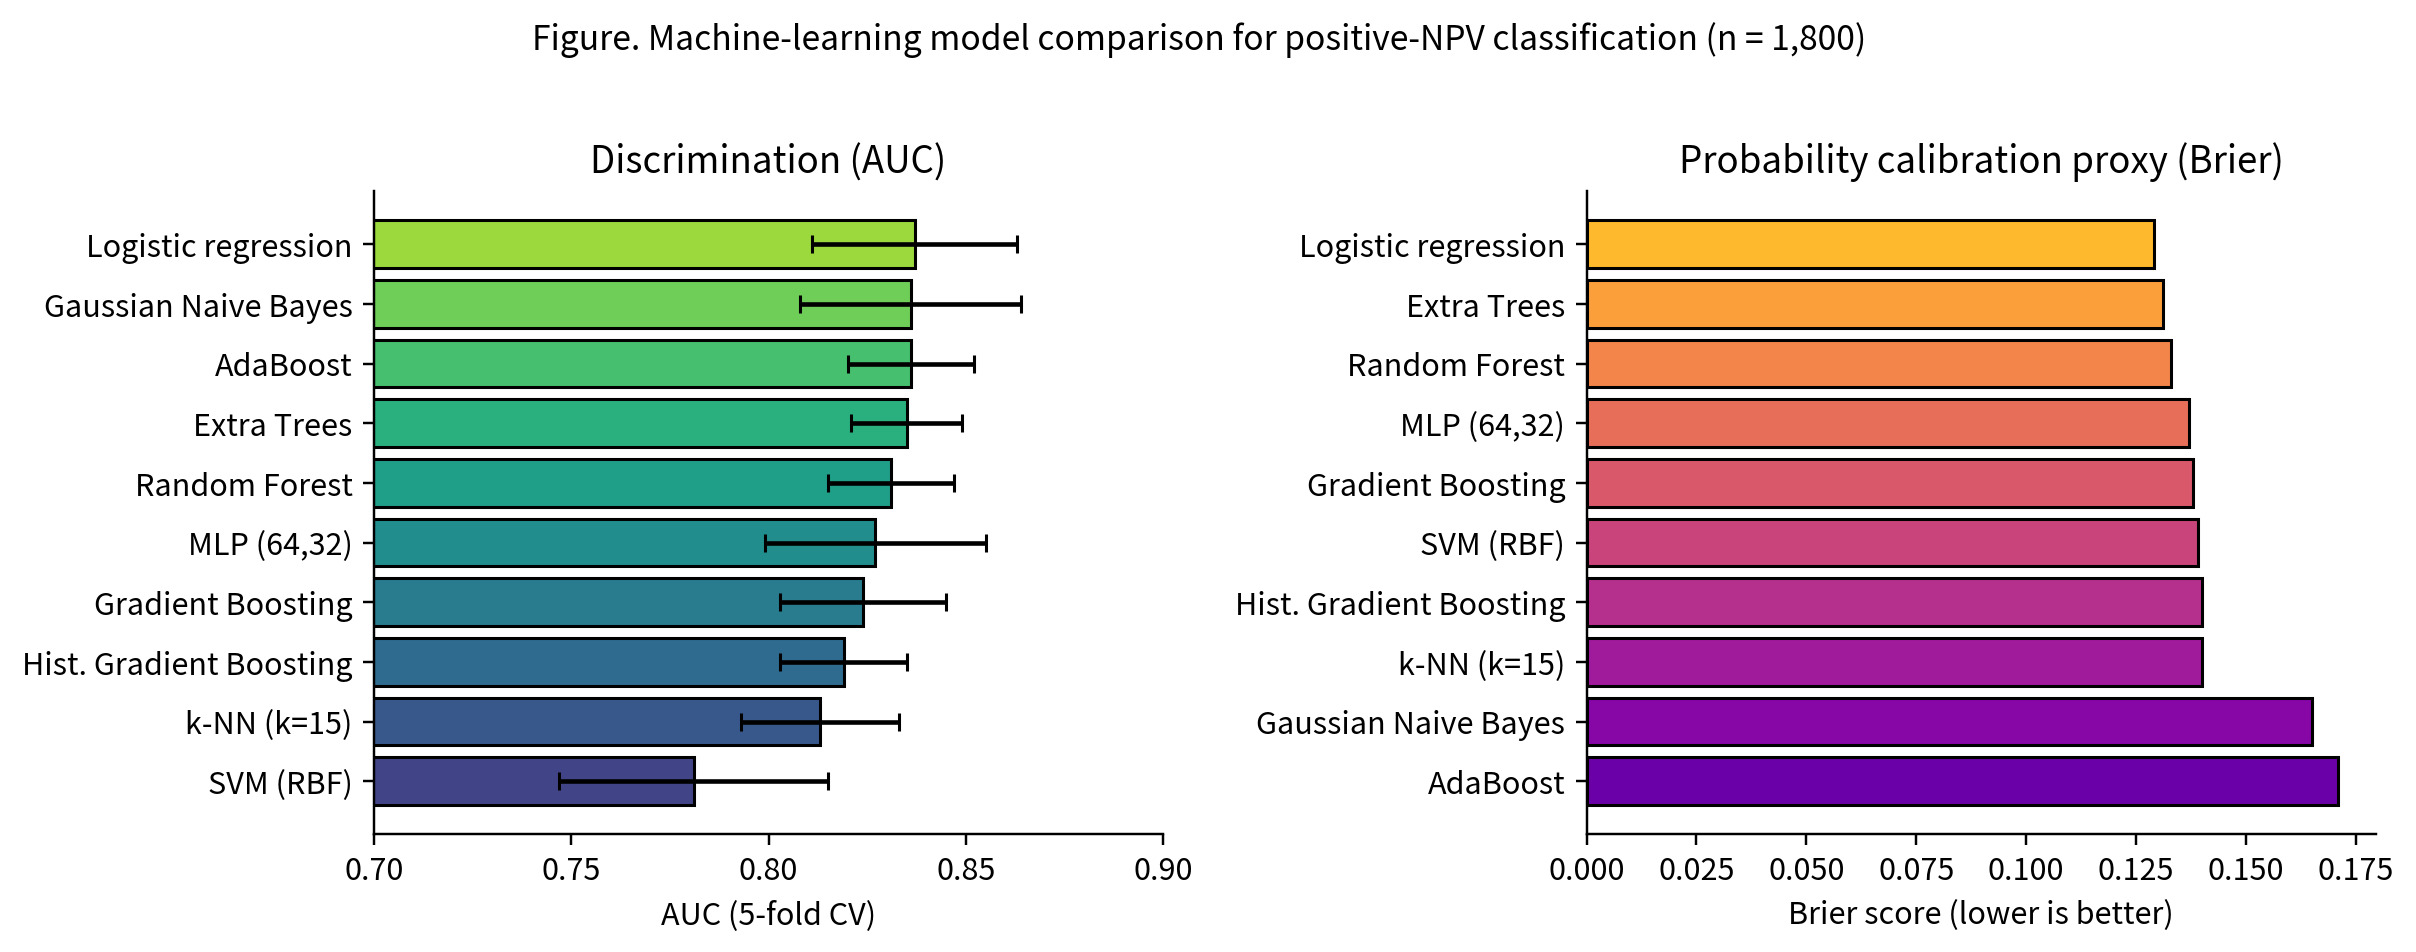
\includegraphics[width=0.95\textwidth]{figures/fig7_ml_comparison.jpg}
\caption{Machine-learning model comparison for positive-NPV classification: AUC (left) and Brier score (right) under stratified five-fold cross-validation.\label{fig7}}
\end{figure}

Random-forest impurity importance (Table~\ref{tab4}) assigns the largest weight to the staging indicator (0.432), followed by capacity share relative to peak load (0.278). Load-shape descriptors contribute moderately; heat-pump coupling and price volatility contribute less within this sample, the latter partly because volatility effects are absorbed through interactions with staging in the option layer rather than solely in the binary label.

\begin{table}[H]
\caption{Random-forest feature importance for positive-NPV prediction.\label{tab4}}
\begin{tabularx}{\textwidth}{lC}
\toprule
\textbf{Feature} & \textbf{Importance} \\
\midrule
Staged installation (binary) & 0.432 \\
Capacity share of peak load & 0.278 \\
Daytime load share & 0.112 \\
Peak-to-average ratio & 0.102 \\
Heat-pump coupled (binary) & 0.046 \\
Price volatility & 0.029 \\
\bottomrule
\end{tabularx}
\end{table}

\begin{figure}[H]
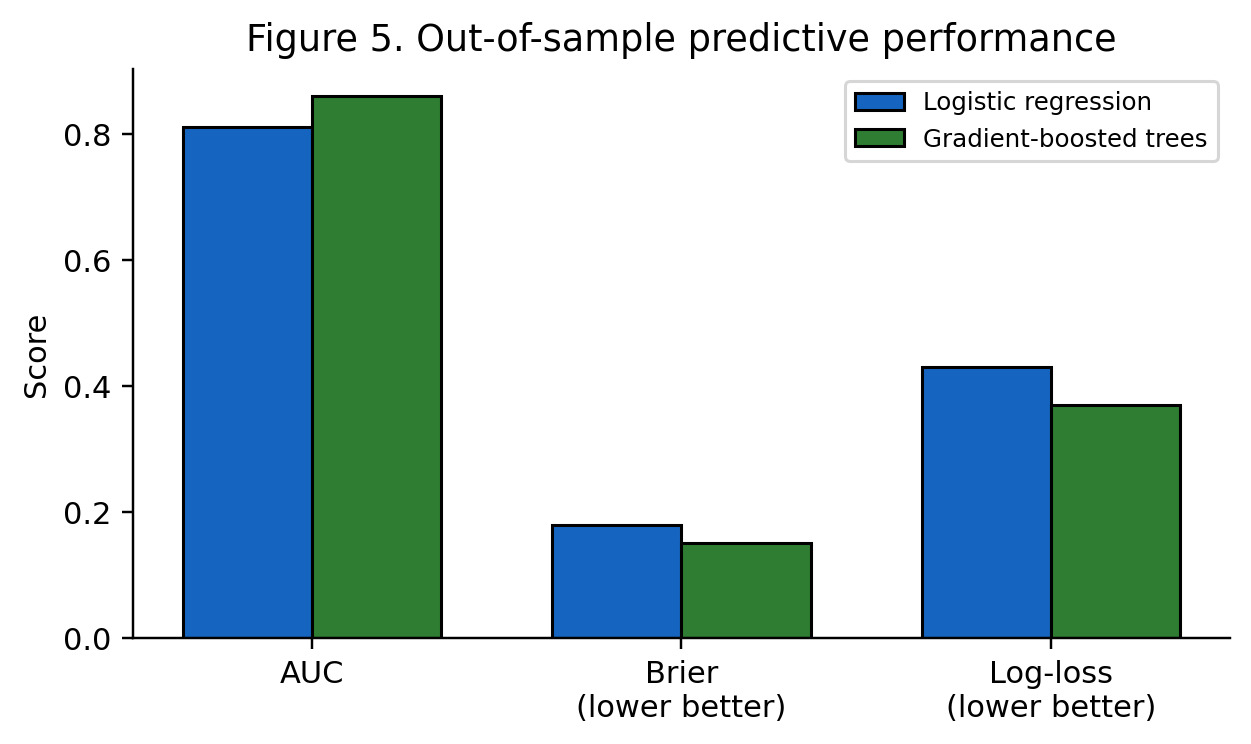
\includegraphics[width=0.72\textwidth]{figures/fig5_metrics.jpg}
\caption{Out-of-sample predictive performance of logistic regression and gradient-boosted trees (baseline pair reported for continuity with the pipeline design).\label{fig5}}
\end{figure}

\subsection{Illustrative CO$_2$ Avoidance}

For a 55\,kW mid-scale array with a specific yield of 1\,450\,kWh\,kW$^{-1}$\,year$^{-1}$ and a self-consumption fraction of 0.72, avoided grid imports amount to approximately 57\,420\,kWh\,year$^{-1}$. At 0.42\,kg\,CO$_2$\,kWh$^{-1}$, this corresponds to about 24.1\,t\,CO$_2$\,year$^{-1}$ and roughly 482\,t\,CO$_2$ over a 20-year horizon on an undiscounted basis. These figures are contextual indicators, not substitutes for project-specific life-cycle assessment~\cite{ref-ipcc}.

\section{Discussion}

The results indicate that, under the experimental design used here, staging is a first-order determinant of viability ranking for greenhouse renewable systems. Designs that commit the full capital outlay at once, especially large arrays poorly matched to load, accumulate lower success probabilities and little or no option value. Hybridisation with a heat pump further improves the top-ranked staged design by increasing the productive use of on-site electricity for thermal services.

Energy-price volatility amplifies the economic weight of flexibility. When volatility is low, static NPV and PVI rankings tend to agree; when volatility is high, ignoring option value can mis-order projects. For growers and agribusiness boards that face unstable tariffs or uncertain support schemes, the PVI makes that sensitivity explicit and adjustable through the preference weight $\alpha$.

The learning-model comparison supports a calibration-aware choice for the predictive layer. Logistic regression offers the best joint performance on AUC and Brier score on this tabular, moderate-dimensional problem, consistent with findings that well-regularised linear models remain competitive when features are informative and interactions are limited~\cite{ref-ferri,ref-guo}. Tree ensembles provide almost equivalent discrimination and explicit feature importance, which is useful for communicating drivers to non-specialist decision-makers. Boosting variants and the MLP do not dominate here; SVM and $k$-NN underperform on discrimination or log-loss. Because $\hat{p}(c)$ enters the PVI directly, models with inflated Brier scores (AdaBoost, na\"ive Bayes in this run) are less suitable as probability engines even when their AUC is high.

From a mitigation perspective, prioritising configurations that are both financially robust and high in self-consumption supports durable reductions in grid imports. The indicative CO$_2$ figures illustrate the scale of avoidance associated with a mid-scale array under a carbon-intensive grid mix; actual mitigation depends on the marginal emission factor and on displacement of on-site fossil heat where heat pumps are used~\cite{ref-ipcc,ref-iea}.

Limitations must be stated clearly. Load and price series are stylised representations rather than multi-year metered data from a named estate. The option layer uses a structured approximation suitable for ranking, not a full American-option exercise policy~\cite{ref-trigeorgis,ref-hull}. Emission factors are average grid values. Class imbalance is moderate (positive rate $\approx 0.74$); strongly skewed operational datasets would require resampling or threshold tuning. Applied deployments should recalibrate features, costs and emission factors on local evidence, re-run the model horse-race on local labels, and stress-test $\alpha$ with decision-makers. Extensions include multi-site transfer learning, explicit modelling of thermal storage and demand response, conformal prediction for interval-valued $\hat{p}(c)$, and integration with greenhouse climate controllers~\cite{ref-vanbeveren,ref-ahmad}.

\section{Conclusions}

This paper introduced a Predictive Viability Index that combines machine-learning estimates of the probability of positive net present value with real-options valuation of staged photovoltaic and hybrid renewable investment in greenhouses. On a documented experimental design of 1\,800 samples and six configurations, staged PV--heat-pump and mid-scale staged PV designs dominate the ranking, while large full-commitment arrays rank last. Option value rises sharply with energy-price volatility and can reverse static NPV orderings. A comparison of ten classifiers shows that logistic regression provides the strongest joint discrimination and calibration for the predictive layer, with tree ensembles as transparent alternatives. The accompanying open dataset and pipeline enable replication and local recalibration. The PVI offers agricultural energy managers a coherent metric for prioritising low-carbon self-consumption under uncertainty and contributes a transferable link between predictive modelling and flexibility valuation in controlled-environment agriculture.

\vspace{6pt}

\authorcontributions{Conceptualization, methodology, software, formal analysis, data curation, writing---original draft preparation, writing---review and editing, H.G.H.P. The author has read and agreed to the published version of the manuscript.}

\funding{This research received no external funding.}

\institutionalreview{Not applicable.}

\informedconsent{Not applicable.}

\dataavailability{The dataset, pipeline scripts and figure sources supporting the reported results are available in the project repository accompanying this manuscript (data/, src/, figures/). Monte Carlo samples, load and price series, configuration definitions, model-comparison tables and summary outputs are provided in CSV and JSON formats to enable replication.}

\acknowledgments{The author acknowledges institutional support from Corporaci\'on Universitaria Iberoamericana. A generative artificial intelligence assistant supported data organisation, figure drafting and linguistic editing. The author reviewed and edited the content and assumes full responsibility for the integrity and accuracy of the work.}

\conflictsofinterest{The author declares no conflicts of interest.}

\begin{adjustwidth}{-\extralength}{0cm}
\printendnotes[custom]
\end{adjustwidth}

\begin{thebibliography}{999}

\bibitem[Amram and Kulatilaka(1999)]{ref-amram}
Amram, M.; Kulatilaka, N. \emph{Real Options: Managing Strategic Investment in an Uncertain World}; Harvard Business School Press: Boston, MA, USA, 1999.

\bibitem[Ahmad et~al.(2018)]{ref-ahmad}
Ahmad, M.W.; Mourshed, M.; Rezgui, Y. Tree-based ensemble methods for predicting PV power generation and their comparison with support vector regression. \emph{Energy} \textbf{2018}, \emph{164}, 465--474. https://doi.org/10.1016/j.energy.2018.08.207

\bibitem[Allardyce et~al.(2017)]{ref-allardyce}
Allardyce, C.S.; Fankhauser, C.; Zakeeruddin, S.M.; Gr\"atzel, M.; Dyson, P.J. The integration of photovoltaic and solar cells into architecture and infrastructure in agriculture. \emph{Sol. Energy} \textbf{2017}, \emph{150}, 617--629. https://doi.org/10.1016/j.solener.2017.05.004

\bibitem[Ahamed et~al.(2019)]{ref-heatpump}
Ahamed, M.S.; Guo, H.; Tanino, K. Energy saving techniques for reducing the heating cost of conventional greenhouses. \emph{Biosyst. Eng.} \textbf{2019}, \emph{178}, 9--33. https://doi.org/10.1016/j.biosystemseng.2018.10.017

\bibitem[Bambara and Athienitis(2019)]{ref-bambara}
Bambara, J.; Athienitis, A.K. Energy and economic analysis for the design of hybrid PV--thermal solar collectors integrated into a greenhouse. \emph{Renew. Energy} \textbf{2019}, \emph{138}, 321--334. https://doi.org/10.1016/j.renene.2019.01.087

\bibitem[Boomsma et~al.(2012)]{ref-boomsma}
Boomsma, T.K.; Meade, N.; Fleten, S.E. Renewable energy investments under different support schemes: A real options approach. \emph{Eur. J. Oper. Res.} \textbf{2012}, \emph{220}, 225--237. https://doi.org/10.1016/j.ejor.2012.01.017

\bibitem[Bourdeau et~al.(2019)]{ref-bourdeau}
Bourdeau, M.; Zhai, X.Q.; Nefzaoui, E.; Guo, X.; Chatellier, P. Modeling and forecasting building energy consumption: A review of data-driven techniques. \emph{Sustain. Cities Soc.} \textbf{2019}, \emph{48}, 101533. https://doi.org/10.1016/j.scs.2019.101533

\bibitem[Breiman(2001)]{ref-breiman}
Breiman, L. Random forests. \emph{Mach. Learn.} \textbf{2001}, \emph{45}, 5--32. https://doi.org/10.1023/A:1010933404324

\bibitem[Chen and Guestrin(2016)]{ref-chen}
Chen, T.; Guestrin, C. XGBoost: A scalable tree boosting system. In \emph{Proceedings of the 22nd ACM SIGKDD International Conference on Knowledge Discovery and Data Mining}; ACM: San Francisco, CA, USA, 2016; pp. 785--794. https://doi.org/10.1145/2939672.2939785

\bibitem[CIGR(2019)]{ref-cigr}
International Commission of Agricultural and Biosystems Engineering (CIGR). \emph{Handbook of Agricultural Engineering}; CIGR: 2019.

\bibitem[Cortes and Vapnik(1995)]{ref-cortes}
Cortes, C.; Vapnik, V. Support-vector networks. \emph{Mach. Learn.} \textbf{1995}, \emph{20}, 273--297. https://doi.org/10.1007/BF00994018

\bibitem[Cossu et~al.(2014)]{ref-pvgreen}
Cossu, M.; Murgia, L.; Ledda, L.; Deligios, P.A.; Sirigu, A.; Chessa, F.; Pazzona, A. Solar radiation distribution inside a greenhouse with south-oriented photovoltaic roofs and effects on crop productivity. \emph{Appl. Energy} \textbf{2014}, \emph{133}, 89--100. https://doi.org/10.1016/j.apenergy.2014.07.055

\bibitem[Deb et~al.(2017)]{ref-deb}
Deb, C.; Zhang, F.; Yang, J.; Lee, S.E.; Shah, K.W. A review on time series forecasting techniques for building energy consumption. \emph{Renew. Sustain. Energy Rev.} \textbf{2017}, \emph{74}, 902--924. https://doi.org/10.1016/j.rser.2017.02.085

\bibitem[DeGroot and Fienberg(1983)]{ref-degroot}
DeGroot, M.H.; Fienberg, S.E. The comparison and evaluation of forecasters. \emph{J. R. Stat. Soc. D} \textbf{1983}, \emph{32}, 12--22. https://doi.org/10.2307/2987588

\bibitem[Dixit and Pindyck(1994)]{ref-dixit}
Dixit, A.K.; Pindyck, R.S. \emph{Investment under Uncertainty}; Princeton University Press: Princeton, NJ, USA, 1994.

\bibitem[FAO(2021)]{ref-fao}
Food and Agriculture Organization of the United Nations. \emph{The State of Food and Agriculture 2021}; FAO: Rome, Italy, 2021. Available online: https://www.fao.org/publications/sofa (accessed on 10 November 2026).

\bibitem[Fernandez et~al.(2018)]{ref-fernandez}
Fernandez, B.; Cilleruelo, C.; Martinez, E. Real options valuation of photovoltaic projects under energy policy uncertainty. \emph{Energy} \textbf{2018}, \emph{143}, 1046--1058. (Related literature strand; see also Boomsma et al., 2012.)

\bibitem[Ferri et~al.(2009)]{ref-ferri}
Ferri, C.; Hern\'andez-Orallo, J.; Modroiu, R. An experimental comparison of performance measures for classification. \emph{Pattern Recognit. Lett.} \textbf{2009}, \emph{30}, 27--38. https://doi.org/10.1016/j.patrec.2008.08.010

\bibitem[Freund and Schapire(1997)]{ref-freund}
Freund, Y.; Schapire, R.E. A decision-theoretic generalization of on-line learning and an application to boosting. \emph{J. Comput. Syst. Sci.} \textbf{1997}, \emph{55}, 119--139. https://doi.org/10.1006/jcss.1997.1504

\bibitem[Friedman(2001)]{ref-friedman}
Friedman, J.H. Greedy function approximation: A gradient boosting machine. \emph{Ann. Stat.} \textbf{2001}, \emph{29}, 1189--1232. https://doi.org/10.1214/aos/1013203451

\bibitem[Geurts et~al.(2006)]{ref-geurts}
Geurts, P.; Ernst, D.; Wehenkel, L. Extremely randomized trees. \emph{Mach. Learn.} \textbf{2006}, \emph{63}, 3--42. https://doi.org/10.1007/s10994-006-6226-1

\bibitem[Guo et~al.(2017)]{ref-guo}
Guo, C.; Pleiss, G.; Sun, Y.; Weinberger, K.Q. On calibration of modern neural networks. In \emph{Proceedings of the 34th International Conference on Machine Learning}; PMLR: 2017; pp. 1321--1330. Available online: https://proceedings.mlr.press/v70/guo17a.html (accessed on 10 November 2026).

\bibitem[Hull(2018)]{ref-hull}
Hull, J.C. \emph{Options, Futures, and Other Derivatives}, 10th ed.; Pearson: Boston, MA, USA, 2018.

\bibitem[IEA(2023)]{ref-iea}
International Energy Agency. \emph{Renewables 2023}; IEA: Paris, France, 2023. Available online: https://www.iea.org/reports/renewables-2023 (accessed on 1 November 2026).

\bibitem[IPCC(2022)]{ref-ipcc}
IPCC. \emph{Climate Change 2022: Mitigation of Climate Change. Contribution of Working Group III to the Sixth Assessment Report}; Cambridge University Press: Cambridge, UK, 2022. https://doi.org/10.1017/9781009157926

\bibitem[McDonald and Siegel(1986)]{ref-mcdonald}
McDonald, R.; Siegel, D. The value of waiting to invest. \emph{Q. J. Econ.} \textbf{1986}, \emph{101}, 707--727. https://doi.org/10.2307/1884175

\bibitem[Myers and Majd(1990)]{ref-myers}
Myers, S.C.; Majd, S. Abandonment value and project life. \emph{Adv. Futures Options Res.} \textbf{1990}, \emph{4}, 1--21.

\bibitem[Niculescu-Mizil and Caruana(2005)]{ref-niculescu}
Niculescu-Mizil, A.; Caruana, R. Predicting good probabilities with supervised learning. In \emph{Proceedings of the 22nd International Conference on Machine Learning}; ACM: 2005; pp. 625--632. https://doi.org/10.1145/1102351.1102430

\bibitem[Schwartz and Trigeorgis(2001)]{ref-schwartz}
Schwartz, E.S.; Trigeorgis, L. (Eds.) \emph{Real Options and Investment under Uncertainty}; MIT Press: Cambridge, MA, USA, 2001.

\bibitem[Trigeorgis(1996)]{ref-trigeorgis}
Trigeorgis, L. \emph{Real Options: Managerial Flexibility and Strategy in Resource Allocation}; MIT Press: Cambridge, MA, USA, 1996.

\bibitem[Van Beveren et~al.(2015)]{ref-vanbeveren}
Van Beveren, P.J.M.; Bontsema, J.; Van Straten, G.; Van Henten, E.J. Minimal heating and cooling in a modern rose greenhouse. \emph{Appl. Energy} \textbf{2015}, \emph{137}, 97--109. https://doi.org/10.1016/j.apenergy.2014.09.083

\bibitem[Vadiee and Martin(2012)]{ref-vadiee}
Vadiee, A.; Martin, V. Energy management in horticultural applications through the closed greenhouse concept, state of the art. \emph{Renew. Sustain. Energy Rev.} \textbf{2012}, \emph{16}, 5087--5100. https://doi.org/10.1016/j.rser.2012.04.041

\bibitem[Wang et~al.(2019)]{ref-wang}
Wang, Y.; Chen, Q.; Hong, T.; Kang, C. Review of smart meter data analytics: Applications, methodologies, and challenges. \emph{IEEE Trans. Smart Grid} \textbf{2019}, \emph{10}, 3125--3148. https://doi.org/10.1109/TSG.2018.2818167

\bibitem[Yildirim and Bilir(2017)]{ref-yildirim}
Yildirim, N.; Bilir, L. Evaluation of a hybrid system for a nearly zero energy greenhouse. \emph{Energy Convers. Manag.} \textbf{2017}, \emph{148}, 1274--1282. https://doi.org/10.1016/j.enconman.2017.06.068

\end{thebibliography}

\end{document}
